\documentclass[12pt]{article}
% # FONTS

\usepackage[T1]{fontenc}
\usepackage{tgtermes}
\usepackage[utf8]{inputenc}

% NOTE: MUST INSTALL SEPARATELY
\usepackage[subscriptcorrection,
           amssymbols,
           mtpbb,
           mtpcal,
           nofontinfo  % suppresses all warnings
          ]{mtpro2}
% NOTE: MUST UNCOMMENT IF NOT USING MTPRO2
%\usepackage{amssymb}
%\newcommand{\mathbold}[1]{\ensuremath{\boldsymbol{\mathbf{#1}}}}

\usepackage{scalefnt,letltxmacro}
\LetLtxMacro{\oldtextsc}{\textsc}
\renewcommand{\textsc}[1]{\oldtextsc{\scalefont{1.10}#1}}
% \renewcommand*\ttdefault{lmvtt}
\usepackage[ttdefault=true]{AnonymousPro}

% # MATH

\usepackage{amsmath}

% # SPACING and TEXT

\usepackage[
  paper  = letterpaper,
  left   = 1.25in,
  right  = 1.25in,
  top    = 1.0in,
  bottom = 1.0in,
  ]{geometry}
% \usepackage[final,expansion=alltext]{microtype}
\usepackage[english]{babel}
\usepackage[parfill]{parskip}
\usepackage{afterpage}
\usepackage{enumitem}
\usepackage{framed}
\usepackage{xspace}

% # EDITING

\renewenvironment{leftbar}[1][\hsize] {%
  \def\FrameCommand {%
    {\color{Gray}\vrule width 3pt}%
    \hspace{10pt}%
    %\hspace{0pt}\fboxsep=\FrameSep\colorbox{black!10}%
  }%
  \MakeFramed{\hsize#1\advance\hsize-\width\FrameRestore}%
}%
{\endMakeFramed}

\usepackage{lineno}
\renewcommand\linenumberfont{\normalfont
                             \footnotesize
                             \sffamily
                             \color{SkyBlue}}

\usepackage{ragged2e}
\DeclareRobustCommand{\sidenote}[1]{\marginpar{
                                    \RaggedRight
                                    \textcolor{Plum}{\textsf{#1}}}}

\newcommand{\parnum}{\bfseries\P\arabic{parcount}}
\newcounter{parcount}
\newcommand\p{%
    \stepcounter{parcount}%
    \leavevmode\marginpar[\hfill\parnum]{\parnum}%
}
\DeclareRobustCommand{\parhead}[1]{\textbf{#1}~}
\setlength{\marginparwidth}{1.0in}

% # COLOR

\usepackage[usenames,dvipsnames]{xcolor}
\definecolor{shadecolor}{gray}{0.9}

\newcommand{\red}[1]{\textcolor{BrickRed}{#1}}
\newcommand{\orange}[1]{\textcolor{BurntOrange}{#1}}
\newcommand{\green}[1]{\textcolor{OliveGreen}{#1}}
\newcommand{\blue}[1]{\textcolor{MidnightBlue}{#1}}
\newcommand{\sky}[1]{\textcolor{SkyBlue}{#1}}
\newcommand{\gray}[1]{\textcolor{black!60}{#1}}

% # COUNTERS

\renewcommand{\labelenumi}{\color{black!67}{\arabic{enumi}.}}
\renewcommand{\labelenumii}{{\color{black!67}(\alph{enumii})}}
\renewcommand{\labelitemi}{{\color{black!67}\textbullet}}

% # FIGURES

\usepackage{graphicx}
\usepackage[labelfont=bf]{caption}
\usepackage{subcaption}

% # TABLES

\usepackage{booktabs,array}

% # ALGORITHMS

\usepackage[algoruled]{algorithm2e}
\setlength{\interspacetitleruled}{8pt}
\usepackage{listings}
\usepackage{fancyvrb}
\fvset{fontsize=\small}

% # BIBLIOGRAPHY AND LINKS

\usepackage{natbib}
\usepackage[colorlinks,linktoc=all]{hyperref}
\usepackage[all]{hypcap}
\hypersetup{citecolor=MidnightBlue}
\hypersetup{linkcolor=MidnightBlue}
\hypersetup{urlcolor=MidnightBlue}

\usepackage[nameinlink]{cleveref}
\crefname{section}{§}{§§}
\Crefname{section}{§}{§§}
\creflabelformat{equation}{#2\textup{#1}#3}  % <- remove parenthesis from equations

% # ACRONYMS

\usepackage
[acronym,smallcaps,nowarn,section,nonumberlist]{glossaries}
\glsdisablehyper{}

% # CODE SNIPPETS

\definecolor{strings}{rgb}{.624,.251,.259}
\definecolor{keywords}{rgb}{.224,.451,.686}
\definecolor{comment}{rgb}{.322,.451,.322}

\usepackage{minted}
\newminted{python}{fontsize=\footnotesize,mathescape=True,escapeinside=@@}

% # USEFUL COMMANDS

\newcommand{\pp}{\textcolor{Plum}{\P\,}}
\newcommand{\q}[1]{\red{{\sf Q | #1}}}
\newcommand{\draftdisclaimer}{\begin{center}\begin{framed} DRAFT: DO
NOT CITE OR DISTRIBUTE \end{framed}\end{center}}

\newacronym{VI}{vi}{variational inference}
\newacronym{KL}{kl}{Kullback-Leibler}
\newacronym{ELBO}{elbo}{\emph{evidence lower bound}}
\newacronym{MCMC}{mcmc}{Markov chain Monte Carlo}

% # PROBABILITY

\newcommand{\g}{\,|\,}
\renewcommand{\gg}{\,\|\,}
\renewcommand{\d}[1]{\ensuremath{\operatorname{d}\!{#1}}}

% # BOLD MATHEMATICS

\newcommand{\mba}{\mathbold{a}}
\newcommand{\mbb}{\mathbold{b}}
\newcommand{\mbc}{\mathbold{c}}
\newcommand{\mbd}{\mathbold{d}}
\newcommand{\mbe}{\mathbold{e}}
%\newcommand{\mbf}{\mathbold{f}}
\newcommand{\mbg}{\mathbold{g}}
\newcommand{\mbh}{\mathbold{h}}
\newcommand{\mbi}{\mathbold{i}}
\newcommand{\mbj}{\mathbold{j}}
\newcommand{\mbk}{\mathbold{k}}
\newcommand{\mbl}{\mathbold{l}}
\newcommand{\mbm}{\mathbold{m}}
\newcommand{\mbn}{\mathbold{n}}
\newcommand{\mbo}{\mathbold{o}}
\newcommand{\mbp}{\mathbold{p}}
\newcommand{\mbq}{\mathbold{q}}
\newcommand{\mbr}{\mathbold{r}}
\newcommand{\mbs}{\mathbold{s}}
\newcommand{\mbt}{\mathbold{t}}
\newcommand{\mbu}{\mathbold{u}}
\newcommand{\mbv}{\mathbold{v}}
\newcommand{\mbw}{\mathbold{w}}
\newcommand{\mbx}{\mathbold{x}}
\newcommand{\mby}{\mathbold{y}}
\newcommand{\mbz}{\mathbold{z}}

\newcommand{\mbA}{\mathbold{A}}
\newcommand{\mbB}{\mathbold{B}}
\newcommand{\mbC}{\mathbold{C}}
\newcommand{\mbD}{\mathbold{D}}
\newcommand{\mbE}{\mathbold{E}}
\newcommand{\mbF}{\mathbold{F}}
\newcommand{\mbG}{\mathbold{G}}
\newcommand{\mbH}{\mathbold{H}}
\newcommand{\mbI}{\mathbold{I}}
\newcommand{\mbJ}{\mathbold{J}}
\newcommand{\mbK}{\mathbold{K}}
\newcommand{\mbL}{\mathbold{L}}
\newcommand{\mbM}{\mathbold{M}}
\newcommand{\mbN}{\mathbold{N}}
\newcommand{\mbO}{\mathbold{O}}
\newcommand{\mbP}{\mathbold{P}}
\newcommand{\mbQ}{\mathbold{Q}}
\newcommand{\mbR}{\mathbold{R}}
\newcommand{\mbS}{\mathbold{S}}
\newcommand{\mbT}{\mathbold{T}}
\newcommand{\mbU}{\mathbold{U}}
\newcommand{\mbV}{\mathbold{V}}
\newcommand{\mbW}{\mathbold{W}}
\newcommand{\mbX}{\mathbold{X}}
\newcommand{\mbY}{\mathbold{Y}}
\newcommand{\mbZ}{\mathbold{Z}}

\newcommand{\mbalpha}{\mathbold{\alpha}}
\newcommand{\mbbeta}{\mathbold{\beta}}
\newcommand{\mbdelta}{\mathbold{\delta}}
\newcommand{\mbepsilon}{\mathbold{\epsilon}}
\newcommand{\mbchi}{\mathbold{\chi}}
\newcommand{\mbeta}{\mathbold{\eta}}
\newcommand{\mbgamma}{\mathbold{\gamma}}
\newcommand{\mbiota}{\mathbold{\iota}}
\newcommand{\mbkappa}{\mathbold{\kappa}}
\newcommand{\mblambda}{\mathbold{\lambda}}
\newcommand{\mbmu}{\mathbold{\mu}}
\newcommand{\mbnu}{\mathbold{\nu}}
\newcommand{\mbomega}{\mathbold{\omega}}
\newcommand{\mbphi}{\mathbold{\phi}}
\newcommand{\mbpi}{\mathbold{\pi}}
\newcommand{\mbpsi}{\mathbold{\psi}}
\newcommand{\mbrho}{\mathbold{\rho}}
\newcommand{\mbsigma}{\mathbold{\sigma}}
\newcommand{\mbtau}{\mathbold{\tau}}
\newcommand{\mbtheta}{\mathbold{\theta}}
\newcommand{\mbupsilon}{\mathbold{\upsilon}}
\newcommand{\mbvarepsilon}{\mathbold{\varepsilon}}
\newcommand{\mbvarphi}{\mathbold{\varphi}}
\newcommand{\mbvartheta}{\mathbold{\vartheta}}
\newcommand{\mbvarrho}{\mathbold{\varrho}}
\newcommand{\mbxi}{\mathbold{\xi}}
\newcommand{\mbzeta}{\mathbold{\zeta}}

\newcommand{\mbDelta}{\mathbold{\Delta}}
\newcommand{\mbGamma}{\mathbold{\Gamma}}
\newcommand{\mbLambda}{\mathbold{\Lambda}}
\newcommand{\mbOmega}{\mathbold{\Omega}}
\newcommand{\mbPhi}{\mathbold{\Phi}}
\newcommand{\mbPi}{\mathbold{\Pi}}
\newcommand{\mbPsi}{\mathbold{\Psi}}
\newcommand{\mbSigma}{\mathbold{\Sigma}}
\newcommand{\mbTheta}{\mathbold{\Theta}}
\newcommand{\mbUpsilon}{\mathbold{\Upsilon}}
\newcommand{\mbXi}{\mathbold{\Xi}}

\newcommand{\mbzero}{\mathbold{0}}
\newcommand{\mbone}{\mathbold{1}}
\newcommand{\mbtwo}{\mathbold{2}}
\newcommand{\mbthree}{\mathbold{3}}
\newcommand{\mbfour}{\mathbold{4}}
\newcommand{\mbfive}{\mathbold{5}}
\newcommand{\mbsix}{\mathbold{6}}
\newcommand{\mbseven}{\mathbold{7}}
\newcommand{\mbeight}{\mathbold{8}}
\newcommand{\mbnine}{\mathbold{9}}

% # DISTRIBUTIONS

\newcommand{\Gam}{\textrm{Gam}}
\newcommand{\InvGam}{\textrm{InvGam}}

% # MISCELLANEOUS

\newcommand{\diag}{\textrm{diag}}
\newcommand{\supp}{\textrm{supp}}
\DeclareMathOperator*{\argmax}{arg\,max}
\DeclareMathOperator*{\argmin}{arg\,min}
\newcommand\indep{\protect\mathpalette{\protect\independenT}{\perp}}
\def\independenT#1#2{\mathrel{\rlap{$#1#2$}\mkern2mu{#1#2}}}

\usepackage{tikz}

\usetikzlibrary{bayesnet} % <- MUST INSTALL SEPARATELY!
% \usetikzlibrary{external}\tikzexternalize

\pgfdeclarelayer{edgelayer}
\pgfdeclarelayer{nodelayer}
\pgfsetlayers{edgelayer,nodelayer,main}

\definecolor{hexcolor0xbfbfbf}{rgb}{0.749,0.749,0.749}

\tikzset{>=latex}
\tikzstyle{none}   = [inner sep=0pt]
\tikzstyle{line}   = [ -, thick, shorten <=1pt, shorten >=1pt ]
\tikzstyle{arrow}  = [ ->, thick, shorten <=1pt, shorten >=1pt ]
\tikzstyle{ardash} = [ dashed, ->, thick, shorten <=1pt, shorten >=1pt ]

\tikzstyle{empty}=[circle,opacity=0.0,text opacity=1.0,inner sep=0pt]
\tikzstyle{box}=[rectangle,fill=White,draw=Black]
\tikzstyle{filled}=[circle,thick,fill=hexcolor0xbfbfbf,draw=Black]
\tikzstyle{hollow}=[circle,thick,fill=White,draw=Black]
\tikzstyle{param}=[rectangle,fill=Black,draw=Black,inner sep=0pt,minimum width=4pt,minimum height=4pt]
\tikzstyle{paramhollow}=[rectangle,thick,fill=White,draw=Black,inner sep=0pt,minimum
width=4pt,minimum height=4pt]

\usepackage{pgfplots}                               % PGFPLOTS baby!
\pgfplotsset{compat=newest}
\pgfplotsset{plot coordinates/math parser=false}
% \usepgfplotslibrary{statistics}
% \usepgfplotslibrary{colorbrewer}                    % <-MUST INSTALL SEPARATELY!
\newlength\figureheight
\newlength\figurewidth
\setlength\figureheight{1.75in}
\setlength\figurewidth{2.5in}


\newlength\figureheightsmall
\newlength\figurewidthsmall
\setlength\figureheightsmall{1.5in}
\setlength\figurewidthsmall{1.85in}

\definecolor{POSTcolor}{rgb}{0.48, 0.20, 0.58} %posterior
\definecolor{Qcolor}{rgb}{0.00, 0.53, 0.22} %q


\title{%
\textbf{Validating Causal Models}
}

\author{
Dustin Tran \\
Columbia University \\
\\
Francisco J.~R.~Ruiz \\
Columbia University \\
\\
Susan Athey \\
Stanford University \\
\\
David M.~Blei \\
Columbia University \\
}

\begin{document}

\maketitle
\bigskip

\begin{abstract}
  The goal of causal inference is to understand the outcome of
  alternative courses of action.  However, all causal inference
  requires assumptions---more so than for standard tasks in
  probabilistic modeling---and testing those assumptions is important
  to assess the validity of a causal model. We develop Bayesian model
  criticism for causal inference, building on the idea of posterior
  predictive checks to assess model fit. Our approach involves
  decomposing the problem, separately criticizing the model of
  treatment assignments and the model of outcomes.  Further we
  discuss how and when we can check the central assumption of
  unconfoundedness, which enables causal statements from observational
  data.  Our approach provides a foundation for diagnosing causal
  inferences from observational data.
\end{abstract}

\emph{Keywords:}
Causal Inference;
Probabilistic Models;
Bayesian Analysis;
Model Checking.

\clearpage
\glsresetall{}

% %!TEX root = Sommerakademie-2015-Forschung.tex
\section{Einleitung}
\subsection{Was ist On-Line Recognition?}

\begin{frame}{Demo}
    \begin{figure}[h]
        \centering
        \includegraphics*[width=0.7\linewidth, keepaspectratio]{images/Classification.png}
    \end{figure}

    \href{http://write-math.com}{write-math.com}
\end{frame}

\begin{frame}{Was ist On-Line Recognition?}
\medskip
\begin{columns}[t,onlytextwidth]
\begin{column}{.5\textwidth}
{\Large Off-line Recognition}
\begin{figure}[h]
    \centering
    \includegraphics*[width=0.7\linewidth, keepaspectratio]{images/A-pixel.png}
\end{figure}
\end{column}
\begin{column}{.5\textwidth}
{\Large On-line Recognition}
\begin{figure}[h]
    \centering
    \includegraphics*[width=0.7\linewidth, keepaspectratio]{images/A-vektor.png}
\end{figure}
\end{column}
\end{columns}
\end{frame}

\begin{frame}{Was wollen wir?}
    \[f(\text{Merkmale}) = \begin{pmatrix}0.7\\ 0.1\\ 0.2\end{pmatrix} = \begin{pmatrix} \mathbb{P}(\gamma)\\ \mathbb{P}(\text{ö})\\ \mathbb{P}(\heartsuit) \end{pmatrix}\]
    \medskip
    \visible<2->{
        \begin{center}
        {\Large Gesucht: Funktion $f$}\\
        (und Merkmalsextraktion)
    }
    \end{center}
\end{frame}

\begin{frame}{Merkmalsextraktion}
    \begin{figure}[h]
        \centering
        \includegraphics*[width=0.7\linewidth, keepaspectratio]{images/A-vektor-merkmalsbildung.png}
    \end{figure}

    Merkmalsvektor fester Länge ist praktisch
\end{frame}

\section{Funktionen}
\subsection{Funktionen}

\begin{frame}{Funktionen}
\begin{figure}[h]
    \centering
    \includegraphics*[width=0.7\linewidth, keepaspectratio]{images/function-machine.png}
\end{figure}
\end{frame}
\begin{frame}{Funktionen}
    \medskip
    \begin{columns}[t,onlytextwidth]
    \begin{column}{.5\textwidth}{
        \begin{itemize}[<+->]
            \item $f(x) = x^2$ ist $f: \mathbb{R} \rightarrow \mathbb{R}$
            \item $f(x, y) = x^2 + y^2$ ist $f: \mathbb{R}^2 \rightarrow \mathbb{R}$
            \item $f(x, y) = (x^2 + y^2, x \cdot y)$ ist $f: \mathbb{R}^2 \rightarrow \mathbb{R}^2$
        \end{itemize}
    }
    \end{column}
    \begin{column}{.4\textwidth}
    \only<1>{
        \begin{tikzpicture}
            \begin{axis}[
                legend pos=south west,
                axis x line=middle,
                axis y line=middle,
                grid = major,
                width=6.5cm,
                height=6.5cm,
                grid style={dashed, gray!30},
                xmin=-2,     % start the diagram at this x-coordinate
                xmax= 2,     % end   the diagram at this x-coordinate
                ymin=-0.25,  % start the diagram at this y-coordinate
                ymax= 4.25,  % end   the diagram at this y-coordinate
                axis background/.style={fill=white},
                xlabel=$x \in \mathbb{R}$,
                ylabel=$f(x) \in \mathbb{R}$,
                %xticklabels={-2,-1.6,...,7},
                %yticklabels={-8,-7,...,8},
                tick align=outside,
                minor tick num=-3,
                enlargelimits=true,
                tension=0.08]
              \addplot[domain=-2:2, red, thick,samples=40] {x*x};
            \end{axis}
        \end{tikzpicture}
    }
    \only<2->{
        \pgfplotsset{
            colormap={whitered}{
                color(0cm)=(white);
                color(1cm)=(orange!75!red)
            }
        }
        \begin{tikzpicture}
            \begin{axis}[
            colormap name=whitered,
            width=5.5cm,
            height=5.5cm,
            view={340}{25},
            enlargelimits=false,
            grid=major,
            domain=-3:3,
            y domain=-3:3,
            samples=56, %57 : TeX capacity exceeded, sorry [main memory size=3000000].
                        % see also http://tex.stackexchange.com/a/7954/5645
            xlabel=$x$,
            ylabel=$y$,
            zlabel={$f(x,y)$},
            ]
              \addplot3[surf] {x^2 + y^2};
            \end{axis}
        \end{tikzpicture}
    }
    \end{column}
    \end{columns}
\end{frame}

\begin{frame}{Funktionen mit Parametern}
    \begin{columns}
    \begin{column}{.5\textwidth}
        {\Large Mit Parametern}
        \begin{itemize}[<+->]
            \item $f(x) = x^2$
            \item $f(x) = 2 \cdot x^2$
            \item $f(x) = \nicefrac{1}{2} \cdot x^2$
            \item $f(x) = a \cdot x^2$
            \item $f(x_1, \dots, x_{166}) = \sum_{i=1}^{166} a_i \cdot x_i$\\
                  $\mathbb{R}^{166} \rightarrow \mathbb{R}$
            \item $f(x_1, \dots, x_{166}) = (\sum_{i=1}^{166} a_i \cdot x_i, \dots, \sum_{i=1}^{166} z_i \cdot x_i)$\\
                  $\mathbb{R}^{166} \rightarrow \mathbb{R}^{\text(\# Klassen)}$
        \end{itemize}
    \end{column}
    \begin{column}{.4\textwidth}
        \begin{tikzpicture}
            \begin{axis}[
                legend pos=south west,
                axis x line=middle,
                axis y line=middle,
                grid = major,
                width=6.5cm,
                height=6.5cm,
                grid style={dashed, gray!30},
                xmin=-2,     % start the diagram at this x-coordinate
                xmax= 2,     % end   the diagram at this x-coordinate
                ymin=-0.25,  % start the diagram at this y-coordinate
                ymax= 4.25,  % end   the diagram at this y-coordinate
                axis background/.style={fill=white},
                xlabel=$x \in \mathbb{R}$,
                ylabel=$f(x) \in \mathbb{R}$,
                %xticklabels={-2,-1.6,...,7},
                %yticklabels={-8,-7,...,8},
                tick align=outside,
                minor tick num=-3,
                enlargelimits=true,
                tension=0.08]
              \only<1->{\addplot[domain=-2:2, red, thick,samples=40] {x*x};}
              \only<2->{\addplot[domain=-2:2, blue, thick,samples=40] {2*x*x};}
              \only<3->{\addplot[domain=-2:2, green, thick,samples=40] {0.5*x*x};}
            \end{axis}
        \end{tikzpicture}
    \end{column}
    \end{columns}
\end{frame}

\begin{frame}{Fehlerfunktion}
    \begin{itemize}[<+->]
        \item \textbf{Daten $(x_{i,1}, \dots, x_{i,n}, y_{i,1}, \dots, y_{i,\text{\# Klassen}})$}: Beispiele für den Computer
        \item \textbf{Aktuelles Modell $f$}: Funktion mit vielen Parametern
        \item \textbf{Fehlerfunktion}: Wie gut ist $f$ für die vorhandenen
              Daten?
    \end{itemize}
\end{frame}

\begin{frame}{Fehlerfunktion}
    Abbildung von \textbf{Parameterraum} auf den Fehler ($\mathbb{R}_0^+$)
\end{frame}

\begin{frame}{Minimieren mit Ableitungen}
    \begin{figure}[h]
        \centering
        \includegraphics*[width=0.7\linewidth, keepaspectratio]{images/derivative-function.png}
    \end{figure}
\end{frame}

\begin{frame}{Gradientenabstieg}
    \begin{figure}[h]
        \centering
        \includegraphics*[width=0.7\linewidth, keepaspectratio]{images/gradient-descent.png}
    \end{figure}
\end{frame}


\section{Neuronale Netze}
\subsection{Neuronale Netze}
\begin{frame}{Neuronale Netze}{}
    \begin{itemize}[<+->]
        \item Menge von parametrisierten Funktionen
              $\mathbb{R}^n \rightarrow \mathbb{R}^{\text(\# Klassen)}$
        \item $\mathbb{R}^n$: Eingabe,\\z.B. Farbe von Pixel~1, Farbe von Pixel~2, \dots
        \item $\mathbb{R}^{\text(\# Klassen)}$: Ausgabe,\\Wahrscheinlichkeit der Klasse (z.B. 0, 1, 2, 3, 4, 5, 6, 7, 8, 9)
        \item Ableitbar
    \end{itemize}
\end{frame}

\section{Ausblick}
\subsection{Ausblick}
\begin{frame}{Ausblick}
    Erkennung von Formeln
    \begin{itemize}[<+->]
        \item Aufbau eines Sprachmodells der Mathematik
        \item Erweiterung der Symboldatenbank
        \item Segmentierung
    \end{itemize}
\end{frame}



\clearpage
\bibliographystyle{apalike}
\bibliography{bib}
\clearpage
\appendix
% %!TEX root = main.tex

\appendix
\section*{Obtaining the data}
The data can be found at \dbDownloadURL. It is a \verb+tar.gz+ file of
\SI{\dbSizeMB}{\mega\byte}. The file can be verified with the MD5sum

\texttt{\dbMDfivesum}

The data is published under the ODbL~license. If you use
the \dbName~dataset, please cite this paper.

The \verb+tar.gz+ archive contains all data as png images and CSV files with
labels. The CSV files have the
columns \verb+path,symbol_id,latex,user_id+ with a header row. The \verb+path+ is the
relative path to a training example to the CSV file, e.g. \verb+../hasy-data/v2-00000.png+. The
\verb+symbol_id+ is an internal numeric identifier for the symbol class. The
website \href{http://write-math.com/symbol/?id=968}{write-math.com/symbol/?id=[symbol\_id]}
gives information related to the symbol. The column \verb+latex+ contains the
\LaTeX{} command associated with the class.
\onecolumn
%!TEX root = "../thesis.tex"
\section*{Symbol Classes}
            \begin{longtable}{lc|lc}
                \toprule
                \LaTeX & Rendered & \LaTeX & Rendered \\
                \midrule
                \endhead
                \hline \multicolumn{4}{r}{{Continued on next page}} \\
                \endfoot
                \bottomrule
                \caption{112 symbols of \dbName.}
                \endlastfoot
\verb+\&+ & $\&$ &\verb+\nmid+ & $\nmid$\\
\verb+\Im+ & $\Im$ &\verb+\nvDash+ & $\nvDash$\\
\verb+\Re+ & $\Re$ &\verb+\int+ & $\int$\\
\verb+\S+ & $\S$ &\verb+\fint+ & $\fint$\\
\verb+\Vdash+ & $\Vdash$ &\verb+\odot+ & $\odot$\\
\verb+\aleph+ & $\aleph$ &\verb+\oiint+ & $\oiint$\\
\verb+\amalg+ & $\amalg$ &\verb+\oint+ & $\oint$\\
\verb+\angle+ & $\angle$ &\verb+\varoiint+ & $\varoiint$\\
\verb+\ast+ & $\ast$ &\verb+\ominus+ & $\ominus$\\
\verb+\asymp+ & $\asymp$ &\verb+\oplus+ & $\oplus$\\
\verb+\backslash+ & $\backslash$ &\verb+\otimes+ & $\otimes$\\
\verb+\between+ & $\between$ &\verb+\parallel+ & $\parallel$\\
\verb+\blacksquare+ & $\blacksquare$ &\verb+\parr+ & $\parr$\\
\verb+\blacktriangleright+ & $\blacktriangleright$ &\verb+\partial+ & $\partial$\\
\verb+\bot+ & $\bot$ &\verb+\perp+ & $\perp$\\
\verb+\bowtie+ & $\bowtie$ &\verb+\pitchfork+ & $\pitchfork$\\
\verb+\boxdot+ & $\boxdot$ &\verb+\pm+ & $\pm$\\
\verb+\boxplus+ & $\boxplus$ &\verb+\prime+ & $\prime$\\
\verb+\boxtimes+ & $\boxtimes$ &\verb+\prod+ & $\prod$\\
\verb+\bullet+ & $\bullet$ &\verb+\propto+ & $\propto$\\
\verb+\checkmark+ & $\checkmark$ &\verb+\rangle+ & $\rangle$\\
\verb+\circ+ & $\circ$ &\verb+\rceil+ & $\rceil$\\
\verb+\circledR+ & $\circledR$ &\verb+\rfloor+ & $\rfloor$\\
\verb+\circledast+ & $\circledast$ &\verb+\rrbracket+ & $\rrbracket$\\
\verb+\circledcirc+ & $\circledcirc$ &\verb+\rtimes+ & $\rtimes$\\
\verb+\clubsuit+ & $\clubsuit$ &\verb+\sharp+ & $\sharp$\\
\verb+\coprod+ & $\coprod$ &\verb+\sphericalangle+ & $\sphericalangle$\\
\verb+\copyright+ & $\copyright$ &\verb+\sqcap+ & $\sqcap$\\
\verb+\dag+ & $\dag$ &\verb+\sqcup+ & $\sqcup$\\
\verb+\dashv+ & $\dashv$ &\verb+\sqrt{}+ & $\sqrt{}$\\
\verb+\diamond+ & $\diamond$ &\verb+\square+ & $\square$\\
\verb+\diamondsuit+ & $\diamondsuit$ &\verb+\star+ & $\star$\\
\verb+\div+ & $\div$ &\verb+\sum+ & $\sum$\\
\verb+\ell+ & $\ell$ &\verb+\times+ & $\times$\\
\verb+\flat+ & $\flat$ &\verb+\top+ & $\top$\\
\verb+\frown+ & $\frown$ &\verb+\triangle+ & $\triangle$\\
\verb+\guillemotleft+ & $\guillemotleft$ &\verb+\triangledown+ & $\triangledown$\\
\verb+\hbar+ & $\hbar$ &\verb+\triangleleft+ & $\triangleleft$\\
\verb+\heartsuit+ & $\heartsuit$ &\verb+\trianglelefteq+ & $\trianglelefteq$\\
\verb+\infty+ & $\infty$ &\verb+\triangleq+ & $\triangleq$\\
\verb+\langle+ & $\langle$ &\verb+\triangleright+ & $\triangleright$\\
\verb+\lceil+ & $\lceil$ &\verb+\uplus+ & $\uplus$\\
\verb+\lfloor+ & $\lfloor$ &\verb+\vDash+ & $\vDash$\\
\verb+\lhd+ & $\lhd$ &\verb+\varnothing+ & $\varnothing$\\
\verb+\lightning+ & $\lightning$ &\verb+\varpropto+ & $\varpropto$\\
\verb+\llbracket+ & $\llbracket$ &\verb+\vartriangle+ & $\vartriangle$\\
\verb+\lozenge+ & $\lozenge$ &\verb+\vdash+ & $\vdash$\\
\verb+\ltimes+ & $\ltimes$ &\verb+\with+ & $\with$\\
\verb+\mathds{1}+ & $\mathds{1}$ &\verb+\wp+ & $\wp$\\
\verb+\mathsection+ & $\mathsection$ &\verb+\wr+ & $\wr$\\
\verb+\mid+ & $\mid$ &\verb+\{+ & $\{$\\
\verb+\models+ & $\models$ &\verb+\|+ & $\|$\\
\verb+\mp+ & $\mp$ &\verb+\}+ & $\}$\\
\verb+\multimap+ & $\multimap$ &\verb+\vee+ & $\vee$\\
\verb+\nabla+ & $\nabla$ &\verb+\wedge+ & $\wedge$\\
\verb+\neg+ & $\neg$ &\verb+\barwedge+ & $\barwedge$
    \label{table:symbols-of-db-0}
    \end{longtable}


\begin{table}[ht]
        \centering

            \begin{tabular}{lc|lc|lc|lc}
                \toprule
                \LaTeX & Rendered & \LaTeX & Rendered & \LaTeX & Rendered & \LaTeX & Rendered \\
                \midrule
\verb+\#+ & $\#$ &\verb+A+ & $A$ &\verb+S+ & $S$ &\verb+i+ & $i$\\
\verb+\$+ & $\$$ &\verb+B+ & $B$ &\verb+T+ & $T$ &\verb+j+ & $j$\\
\verb+\%+ & $\%$ &\verb+C+ & $C$ &\verb+U+ & $U$ &\verb+k+ & $k$\\
\verb+++ & $+$ &\verb+D+ & $D$ &\verb+V+ & $V$ &\verb+l+ & $l$\\
\verb+-+ & $-$ &\verb+E+ & $E$ &\verb+W+ & $W$ &\verb+m+ & $m$\\
\verb+/+ & $/$ &\verb+F+ & $F$ &\verb+X+ & $X$ &\verb+n+ & $n$\\
\verb+0+ & $0$ &\verb+G+ & $G$ &\verb+Y+ & $Y$ &\verb+o+ & $o$\\
\verb+1+ & $1$ &\verb+H+ & $H$ &\verb+Z+ & $Z$ &\verb+p+ & $p$\\
\verb+2+ & $2$ &\verb+I+ & $I$ &\verb+[+ & $[$ &\verb+q+ & $q$\\
\verb+3+ & $3$ &\verb+J+ & $J$ &\verb+]+ & $]$ &\verb+r+ & $r$\\
\verb+4+ & $4$ &\verb+K+ & $K$ &\verb+a+ & $a$ &\verb+s+ & $s$\\
\verb+5+ & $5$ &\verb+L+ & $L$ &\verb+b+ & $b$ &\verb+u+ & $u$\\
\verb+6+ & $6$ &\verb+M+ & $M$ &\verb+c+ & $c$ &\verb+v+ & $v$\\
\verb+7+ & $7$ &\verb+N+ & $N$ &\verb+d+ & $d$ &\verb+w+ & $w$\\
\verb+8+ & $8$ &\verb+O+ & $O$ &\verb+e+ & $e$ &\verb+x+ & $x$\\
\verb+9+ & $9$ &\verb+P+ & $P$ &\verb+f+ & $f$ &\verb+y+ & $y$\\
\verb+<+ & $<$ &\verb+Q+ & $Q$ &\verb+g+ & $g$ &\verb+z+ & $z$\\
\verb+>+ & $>$ &\verb+R+ & $R$ &\verb+h+ & $h$ &\verb+|+ & $|$\\

        \bottomrule
    \end{tabular}

    \caption{72 ASCII symbols of \dbName, including all
             ten digits, the Latin alphabet in lower and upper case and
             a few more symbols.}
    \label{table:symbols-of-db-1}
\end{table}


\begin{table}[ht]
        \centering
            \begin{tabular}{lc|lc|lc}
                \toprule
                \LaTeX & Rendered & \LaTeX & Rendered & \LaTeX & Rendered \\
                \midrule
\verb+\approx+ & $\approx$ &\verb+\geqslant+ & $\geqslant$ &\verb+\lesssim+ & $\lesssim$\\
\verb+\doteq+ & $\doteq$ &\verb+\neq+ & $\neq$ &\verb+\backsim+ & $\backsim$\\
\verb+\simeq+ & $\simeq$ &\verb+\not\equiv+ & $\not\equiv$ &\verb+\sim+ & $\sim$\\
\verb+\equiv+ & $\equiv$ &\verb+\preccurlyeq+ & $\preccurlyeq$ &\verb+\succ+ & $\succ$\\
\verb+\geq+ & $\geq$ &\verb+\preceq+ & $\preceq$ &\verb+\prec+ & $\prec$\\
\verb+\leq+ & $\leq$ &\verb+\succeq+ & $\succeq$ &\verb+\gtrless+ & $\gtrless$\\
\verb+\leqslant+ & $\leqslant$ &\verb+\gtrsim+ & $\gtrsim$ &\verb+\cong+ & $\cong$\\
        \bottomrule
    \end{tabular}

    \caption{21 symbols which are in \dbName and indicate a relationship.}
    \label{table:symbols-of-db-2}
\end{table}


\begin{table}[ht]
        \centering

            \begin{tabular}{lc|lc}
                \toprule
                \LaTeX & Rendered & \LaTeX & Rendered \\
                \midrule
\verb+\Downarrow+ & $\Downarrow$ &\verb+\nrightarrow+ & $\nrightarrow$\\
\verb+\Leftarrow+ & $\Leftarrow$ &\verb+\rightarrow+ & $\rightarrow$\\
\verb+\Leftrightarrow+ & $\Leftrightarrow$ &\verb+\rightleftarrows+ & $\rightleftarrows$\\
\verb+\Longleftrightarrow+ & $\Longleftrightarrow$ &\verb+\rightrightarrows+ & $\rightrightarrows$\\
\verb+\Longrightarrow+ & $\Longrightarrow$ &\verb+\rightsquigarrow+ & $\rightsquigarrow$\\
\verb+\Rightarrow+ & $\Rightarrow$ &\verb+\searrow+ & $\searrow$\\
\verb+\circlearrowleft+ & $\circlearrowleft$ &\verb+\shortrightarrow+ & $\shortrightarrow$\\
\verb+\circlearrowright+ & $\circlearrowright$ &\verb+\twoheadrightarrow+ & $\twoheadrightarrow$\\
\verb+\curvearrowright+ & $\curvearrowright$ &\verb+\uparrow+ & $\uparrow$\\
\verb+\downarrow+ & $\downarrow$ &\verb+\rightharpoonup+ & $\rightharpoonup$\\
\verb+\hookrightarrow+ & $\hookrightarrow$ &\verb+\rightleftharpoons+ & $\rightleftharpoons$\\
\verb+\leftarrow+ & $\leftarrow$ &\verb+\longmapsto+ & $\longmapsto$\\
\verb+\leftrightarrow+ & $\leftrightarrow$ &\verb+\mapsfrom+ & $\mapsfrom$\\
\verb+\longrightarrow+ & $\longrightarrow$ &\verb+\mapsto+ & $\mapsto$\\
\verb+\nRightarrow+ & $\nRightarrow$ &\verb+\leadsto+ & $\leadsto$\\
\verb+\nearrow+ & $\nearrow$ &\verb+\upharpoonright+ & $\upharpoonright$\\

        \bottomrule
    \end{tabular}

    \caption{32 arrow symbols of \dbName.}
    \label{table:symbols-of-db-3}
\end{table}


\begin{table}[ht]
        \centering

            \begin{tabular}{lc|lc|lc}
                \toprule
                \LaTeX & Rendered & \LaTeX & Rendered & \LaTeX & Rendered \\
                \midrule
\verb+\alpha+ & $\alpha$ &\verb+\xi+ & $\xi$ &\verb+\Xi+ & $\Xi$\\
\verb+\beta+ & $\beta$ &\verb+\pi+ & $\pi$ &\verb+\Pi+ & $\Pi$\\
\verb+\gamma+ & $\gamma$ &\verb+\rho+ & $\rho$ &\verb+\Sigma+ & $\Sigma$\\
\verb+\delta+ & $\delta$ &\verb+\sigma+ & $\sigma$ &\verb+\Phi+ & $\Phi$\\
\verb+\epsilon+ & $\epsilon$ &\verb+\tau+ & $\tau$ &\verb+\Psi+ & $\Psi$\\
\verb+\zeta+ & $\zeta$ &\verb+\phi+ & $\phi$ &\verb+\Omega+ & $\Omega$\\
\verb+\eta+ & $\eta$ &\verb+\chi+ & $\chi$ &\verb+\varepsilon+ & $\varepsilon$\\
\verb+\theta+ & $\theta$ &\verb+\psi+ & $\psi$ &\verb+\varkappa+ & $\varkappa$\\
\verb+\iota+ & $\iota$ &\verb+\omega+ & $\omega$ &\verb+\varpi+ & $\varpi$\\
\verb+\kappa+ & $\kappa$ &\verb+\Gamma+ & $\Gamma$ &\verb+\varrho+ & $\varrho$\\
\verb+\lambda+ & $\lambda$ &\verb+\Delta+ & $\Delta$ &\verb+\varphi+ & $\varphi$\\
\verb+\mu+ & $\mu$ &\verb+\Theta+ & $\Theta$ &\verb+\vartheta+ & $\vartheta$\\
\verb+\nu+ & $\nu$ &\verb+\Lambda+ & $\Lambda$ &\verb+ + & $ $\\

        \bottomrule
    \end{tabular}

    \caption{All Greek letters and some variations of Greek letters were
             used for evaluation. 38 of them are in this table, the rest
             is identical to Latin letters.}
    \label{table:symbols-of-db-4}
\end{table}


\begin{table}[ht]
        \centering

            \begin{tabular}{lc|lc|lc}
                \toprule
                \LaTeX & Rendered & \LaTeX & Rendered & \LaTeX & Rendered \\
                \midrule
\verb+\mathcal{A}+ & $\mathcal{A}$ &\verb+\mathcal{T}+ & $\mathcal{T}$ &\verb+\mathds{Z}+ & $\mathds{Z}$\\
\verb+\mathcal{B}+ & $\mathcal{B}$ &\verb+\mathcal{U}+ & $\mathcal{U}$ &\verb+\mathfrak{A}+ & $\mathfrak{A}$\\
\verb+\mathcal{C}+ & $\mathcal{C}$ &\verb+\mathcal{X}+ & $\mathcal{X}$ &\verb+\mathfrak{M}+ & $\mathfrak{M}$\\
\verb+\mathcal{D}+ & $\mathcal{D}$ &\verb+\mathcal{Z}+ & $\mathcal{Z}$ &\verb+\mathfrak{S}+ & $\mathfrak{S}$\\
\verb+\mathcal{E}+ & $\mathcal{E}$ &\verb+\mathbb{H}+ & $\mathbb{H}$ &\verb+\mathfrak{X}+ & $\mathfrak{X}$\\
\verb+\mathcal{F}+ & $\mathcal{F}$ &\verb+\mathbb{N}+ & $\mathbb{N}$ &\verb+\mathscr{A}+ & $\mathscr{A}$\\
\verb+\mathcal{G}+ & $\mathcal{G}$ &\verb+\mathbb{Q}+ & $\mathbb{Q}$ &\verb+\mathscr{C}+ & $\mathscr{C}$\\
\verb+\mathcal{H}+ & $\mathcal{H}$ &\verb+\mathbb{R}+ & $\mathbb{R}$ &\verb+\mathscr{D}+ & $\mathscr{D}$\\
\verb+\mathcal{L}+ & $\mathcal{L}$ &\verb+\mathbb{Z}+ & $\mathbb{Z}$ &\verb+\mathscr{E}+ & $\mathscr{E}$\\
\verb+\mathcal{M}+ & $\mathcal{M}$ &\verb+\mathds{C}+ & $\mathds{C}$ &\verb+\mathscr{F}+ & $\mathscr{F}$\\
\verb+\mathcal{N}+ & $\mathcal{N}$ &\verb+\mathds{E}+ & $\mathds{E}$ &\verb+\mathscr{H}+ & $\mathscr{H}$\\
\verb+\mathcal{O}+ & $\mathcal{O}$ &\verb+\mathds{N}+ & $\mathds{N}$ &\verb+\mathscr{L}+ & $\mathscr{L}$\\
\verb+\mathcal{P}+ & $\mathcal{P}$ &\verb+\mathds{P}+ & $\mathds{P}$ &\verb+\mathscr{P}+ & $\mathscr{P}$\\
\verb+\mathcal{R}+ & $\mathcal{R}$ &\verb+\mathds{Q}+ & $\mathds{Q}$ &\verb+\mathscr{S}+ & $\mathscr{S}$\\
\verb+\mathcal{S}+ & $\mathcal{S}$ &\verb+\mathds{R}+ & $\mathds{R}$ &\verb+ + & $ $\\

        \bottomrule
    \end{tabular}

    \caption{44 variants of Latin letters in \dbName.}
    \label{table:symbols-of-db-5}
\end{table}


\begin{table}[ht]
        \centering

            \begin{tabular}{lc|lc|lc}
                \toprule
                \LaTeX & Rendered & \LaTeX & Rendered & \LaTeX & Rendered \\
                \midrule
\verb+\therefore+ & $\therefore$ &\verb+\cdot+  & $\cdot$  &\verb+\dots+  & $\dots$\\
\verb+\because+   & $\because$   &\verb+\vdots+ & $\vdots$ &\verb+\ddots+ & $\ddots$\\
\verb+\dotsc+     & $\dotsc$     &\verb+ +      &          &\verb+ +      &  \\
        \bottomrule
    \end{tabular}

    \caption{7 symbols that contain only dots in \dbName.}
    \label{table:symbols-of-db-6}
\end{table}


\begin{table}[ht]
        \centering
            \begin{tabular}{lc|lc|lc|lc|lc}
                \toprule
                \LaTeX & R & \LaTeX & R & \LaTeX & R &  \LaTeX & R & \LaTeX & R \\
                \midrule
\verb+\AA+ & {\r A}                                                           &\verb+\L+       & 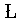
\includegraphics[height=12.3pt, keepaspectratio]{symbols/L.pdf} &\verb+\male+     & {\mbox {\wasyfamily \char 26}}                         &\verb+\ohm+      &  $\Omega $                     &\verb+\sun+       & {\mbox {\wasyfamily \char 46}} \\
\verb+\AE+ & \includegraphics[height=12.3pt, keepaspectratio]{symbols/AE.pdf} &\verb+\O+       & 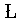
\includegraphics[height=12.3pt, keepaspectratio]{symbols/L.pdf} &\verb+\mars+     & {\leavevmode \lower 0.2ex\hbox {\wasyfamily \char 26}} &\verb+\fullmoon+ & {\mbox {\wasyfamily \char 35}} &\verb+\degree+    & {\ensuremath {^\circ }}\\
\verb+\aa+ & {\r a}                                                           &\verb+\o+       & 
\includegraphics[height=12.3pt, keepaspectratio]{symbols/o.pdf} &\verb+\female+   & {\mbox {\wasyfamily \char 25}}                         &\verb+\leftmoon+ & {\mbox {\wasyfamily \char 36}} &\verb+\iddots+    & 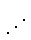
\includegraphics[height=12.3pt, keepaspectratio]{symbols/iddots.pdf}\\
\verb+\ae+ & \includegraphics[height=12.3pt, keepaspectratio]{symbols/AE.pdf} &\verb+\Bowtie+  & {\mbox {\wasyfamily \char 49}}                                  &\verb+\venus+    & {\leavevmode \raise 0.2ex\hbox {\wasyfamily \char 25}} &\verb+\checked+  & {\mbox {\wasyfamily \char 8}}  &\verb+\diameter+  & {\mbox {\wasyfamily \char 31}} \\
\verb+\ss+ & 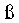
\includegraphics[height=12.3pt, keepaspectratio]{symbols/ss.pdf} &\verb+\celsius+ & $^\circ \mathrm {C}$                                            &\verb+\astrosun+ & {\mbox {$\odot $}}                                     &\verb+\pounds+   & \textsterling                  &\verb+\mathbb{1}+ & 
\includegraphics{symbols/mathbb1.pdf}\\
        \bottomrule
    \end{tabular}
    \caption{25 symbols of \dbName.}
    \label{table:symbols-of-db-7}
\end{table}


\begin{table}[ht]
        \centering

            \begin{tabular}{lc|lc|lc}
                \toprule
                \LaTeX & Rendered & \LaTeX & Rendered & \LaTeX & Rendered \\
                \midrule
\verb+\cup+ & $\cup$ &\verb+\varsubsetneq+ & $\varsubsetneq$ &\verb+\exists+ & $\exists$\\
\verb+\cap+ & $\cap$ &\verb+\nsubseteq+ & $\nsubseteq$ &\verb+\nexists+ & $\nexists$\\
\verb+\emptyset+ & $\emptyset$ &\verb+\sqsubseteq+ & $\sqsubseteq$ &\verb+\forall+ & $\forall$\\
\verb+\setminus+ & $\setminus$ &\verb+\subseteq+ & $\subseteq$ &\verb+\in+ & $\in$\\
\verb+\supset+ & $\supset$ &\verb+\subsetneq+ & $\subsetneq$ &\verb+\ni+ & $\ni$\\
\verb+\subset+ & $\subset$ &\verb+\supseteq+ & $\supseteq$ &\verb+\notin+ & $\notin$\\

        \bottomrule
    \end{tabular}

    \caption{18 set related symbols of \dbName.}
    \label{table:symbols-of-db-8}
\end{table}
\clearpage
\twocolumn

\end{document}
